\documentclass{magic}
\usepackage[ngerman]{babel}
\usepackage[utf8]{inputenc}
\usepackage{standalone}
\usepackage{wrapfig}
\usepackage{graphicx}
\usepackage[locale=DE,range-phrase={ bis }]{siunitx}
\usepackage[shortcuts]{extdash}
\usepackage[ngerman]{babel}
\usepackage{listings}
\usepackage{xcolor}
\usepackage{xfrac}
\usepackage{tikz/magic}
\lstset{language=bash,
  basicstyle=\footnotesize\ttfamily,
	backgroundcolor=\color{mblue!10},
	tabsize=3,
	frame=single,
	rulecolor=\color{mblue!40}
}
\title{MAGIC Datenanalyse}
\subtitle{Lehrstuhlversuch}
\author{E5b}
\date{2018}

\begin{document}
  \maketitle
  Seit der Entdeckung der kosmischen Höhenstrahlung 1912
von Victor Hess feiert die Astroteilchenphysik,
als junge Wissenschaft,
bahnbrechende Errungenschaften.
Mit der Entdeckung der Mikrowellenhintergrundstrahlung 1964,
gilt die Theorie des Urknalls
und eines expandierenden Universums als verifiziert.
Die moderne Astroteilchenphysik beschäftigt sich sowohl mit den
elementaren Bausteinen des Universums,
zum Beispiel durch die Suche nach Dunkler Materie,
als auch mit kosmischen Objekten
und den Beschleunigungsprozessen der emittierten Teilchen
und dessen Sekundärteilchen an sich.
Kosmische Botenteilchen liefern Informationen über
Aktive Galaxienkerne,
Neutronensterne
und weitere kosmische Phänomene,
wie zum Beispiel Supernovae und Gamma Ray Bursts.
Zu den wichtigsten kosmischen Botenteilchen gehören Photonen,
Protonen
und schwerere Kerne,
Neutrinos
und seit der ersten Detektion im Jahr 2015 auch Gravitationswellen.
In diesem Versuch werden die Daten eines Detektors analysiert,
welcher für die Messung von hochenergetischer Gammastrahlung gebaut wurde.

% Seit der Entdeckung der kosmischen Höhenstrahlung
% 1912 von Victor Hess feiert die Astroteilchenphysik bahnbrechende Errungenschaften.
% Die Entdeckung der kosmischen Hintergrundstrahlung gilt als Beleg des
% expandierenden Universums und wirft dennoch weitere Fragen zum frühen Universum auf.
% Durch kosmische Botenteilchen ist das Erforschen von elementaren Bausteine und
% Beschleunigungsprozessen möglich.
% Anhand von kosmischen Botenteilchen können Informationen über Supernovae,
% Aktive Galaxienkerne und weitere kosmische Phänomene, wie zum Beispiel
% Neutronensterne und Gamma Ray Bursts, gewonnen werden.

\section*{MAGIC}%
\label{sec:magic}

\begin{wrapfigure}[13]{O}{0.45\textwidth}
		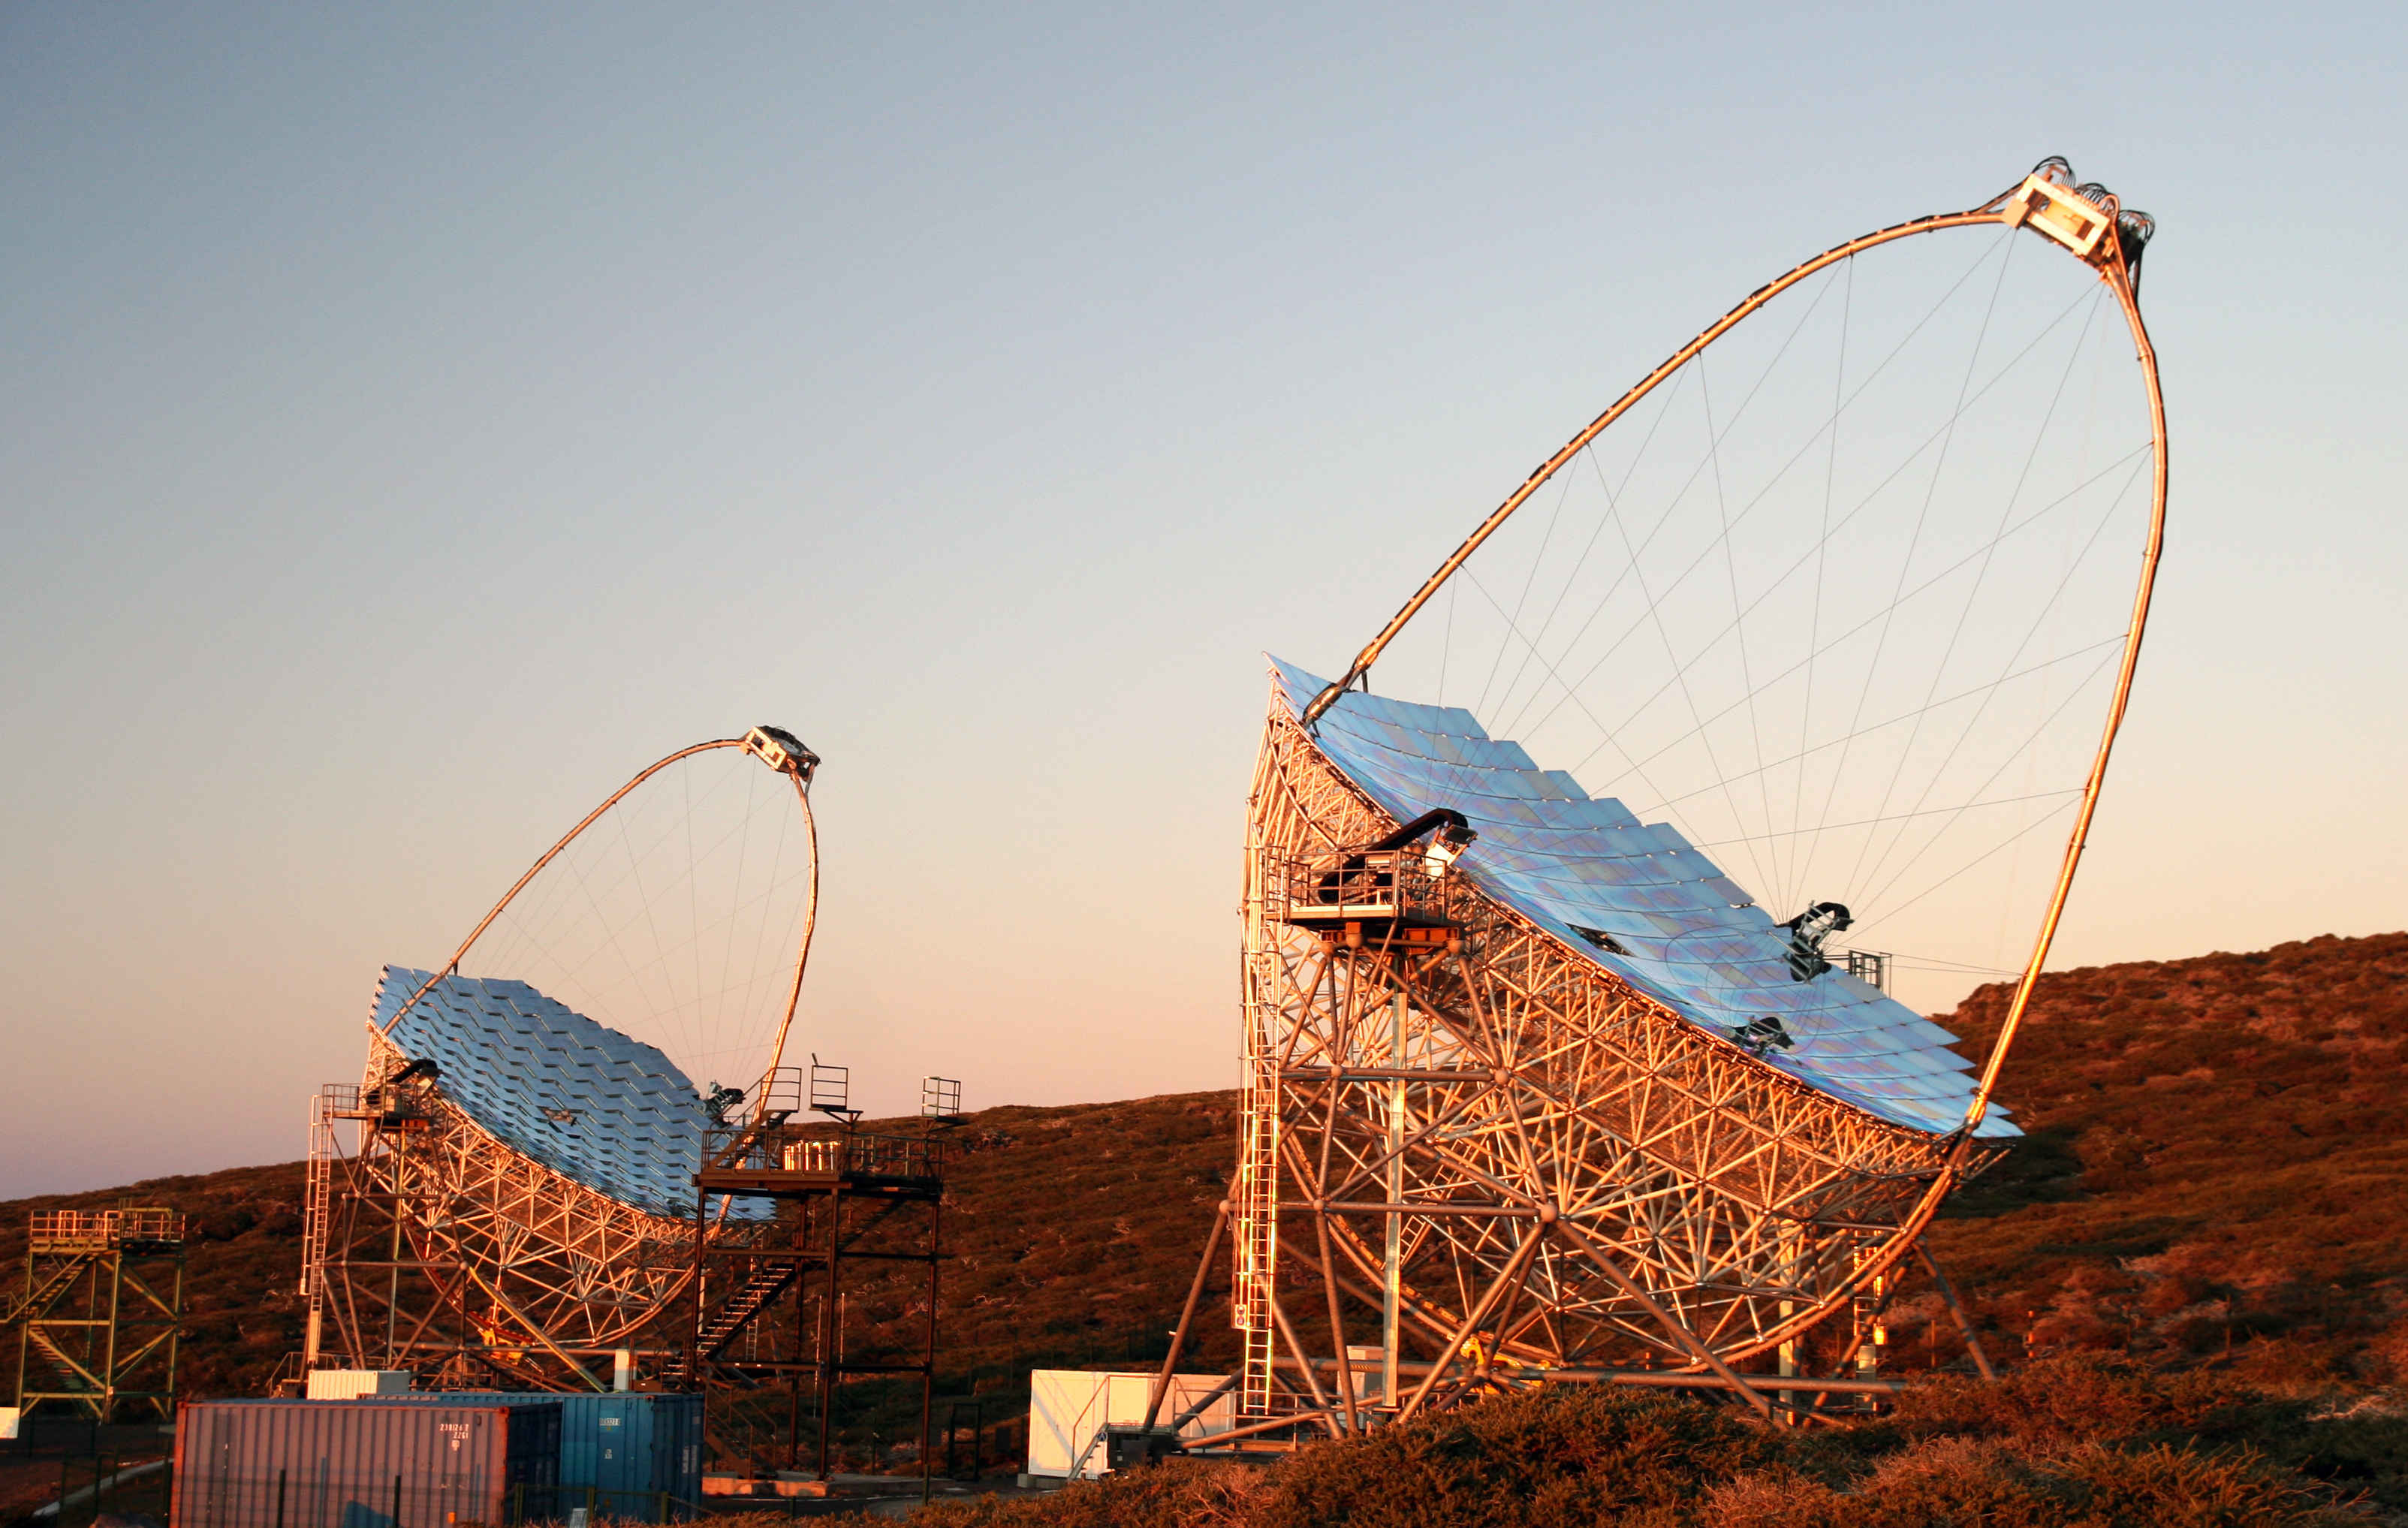
\includegraphics[width=\linewidth]{pictures/magic.JPG}
		\caption{MAGIC Teleskope in Observationsstellung.}%
		\label{fig:magic}
\end{wrapfigure}

% Bitte etwas uebersichtlicher strukturieren, zerst Teleskope, dann Gammas, dann Schauer und dann Tscherenkovlicht:
% Vorschlag:

% Einleitung ok, aber nicht auf Bild verweisen, erst spaeter.

Die \textbf{M}ajor \textbf{A}thmospheric \textbf{G}amma \textbf{I}maging
\textbf{C}herenkov Teleskope (Abbildung \ref{fig:magic}) sind derzeit das
weltweit größte im Stereomodus operierende IACT System.
MAGIC sucht nach Gamma Ray Bursts, beobachtet Blazare und untersucht das
Galaktische Zentrum.
Es befindet sich auf der kanarischen Insel La Palma auf dem Berg 'Roque de Los Muchachos',
in einer Höhe von 2200m über dem Meeresspiegel.
Es ist für Gammastrahlung in einem Energiebereich von
\SI{50}{\giga\electronvolt} bis \SI{50}{\tera\electronvolt} sensitiv.
Beide Teleskope haben eine Spiegelfläche von je \SI{17}{\meter} Durchmesser,
bestehend aus 974 einzelnen Spiegeln,
welche die Schauerbilder auf eine Kamera aus 1039 Photo Multiplier Tubes (PMTs) abbilden.
Der Detektor besitzt ein Sichtfeld von \SI{3,5}{\degree}.

\begin{wrapfigure}[13]{I}{0.45\textwidth}
		\includegraphics[width=\linewidth]{tikz/build/shower.pdf}
		\caption{Teilchen in einem Teilchenschauer mit einem Photon als
    Pri\-mär\-teil\-chen.}%
    \label{fig:schauer}
\end{wrapfigure}
Treten hochenergetische Gammateilchen in die Erdatmosphäre ein,
wechselwirken sie mit den darin enthaltenen Atomkernen
und produzieren durch Paarerzeugung relativistische Elektronen
und Positronen.
Durch Bremsstrahlung werden wiederum relativistische Photonen erzeugt.
Durch das Wechselwirken (Paarerzeugung und Bremsstrahlung) weiterer
Sekundärteilchen entsteht ein Schauer aus Photonen und Leptonen (Abbildung
\ref{fig:schauer}).
Da die geladenen Teilchen im Schauer relativistische Geschwindigkeiten besitzen,
strahlen diese bei der Propagation durch die Atmosphäre Tscherenkowlicht ab.
Ein durch ein in die Erdatmosphäre eintretendes Gammateilchen ausgelöster
Tscherenkowblitz dauert nur einige Nanosekunden
und ist somit mit dem menschlichen Auge nicht erfassbar.

% Der Nachweis von hochenergetischer Gammastrahlung ist auf der Erde aufgrund der
% Atmosphäre nur indirekt möglich.
% Hochenergetische Photonen und Hadronen
% wechselwirken beim Eintritt in die Erdatmosphäre mit dieser
% und erzeugen sogenannte Teilchenschauer,
% eine Kaskade aus wiederum wechselwirkenden Teilchen.
% Aufgrund ihrer relativistischen Geschwindigkeiten
% strahlen geladene Schauerteilchen Tscherenkowlicht ab,
% welches auf der Erde von sehr sensitiven Teleskopen,
% sogenannten IACTs (Imaging Air Cherenkov Telescopes)
% gemessen werden kann.
% erzeugen in der Atmosphäre
% Teilchenschauer (siehe Abbildung~\ref{fig:schauer}), die aufgrund ihrer relativistischen Geschwindigkeiten Tscherenkowlicht abstrahlen.
% \begin{wrapfigure}[13]{I}{0.45\textwidth}
% 		\includegraphics[width=\linewidth]{tikz/build/shower.pdf}
% 		\caption{Teilchen in einem Teilchenschauer mit einem Photon als
%     Pri\-mär\-teil\-chen.}%
%     \label{fig:schauer}
% \end{wrapfigure}
% MAGIC ist derzeit das größte Stereoteleskop,
% welches in einem Energiebereich von \SI{50}{\giga\electronvolt} bis
% \SI{50}{\tera\electronvolt} sensitiv ist.
% Es steht auf der Insel La Palma auf einer Höhe von \SI{2200}{\meter}.
% Propagiert ein geladenes Teilchen mit einer Geschwindigkeit in einem
% Medium, die höher als die Lichtgeschwindigkeit in diesem Medium ist,
% so erzeugt dieses Tscherenkow-Photonen.
% Die ultrarelativistischen Photonen, welche in die Erdatmosphäre eintreten,
% wechselwirken mit den darin enthaltenen Teilchen beispielsweise über
% Bremsstrahlung oder Paarerzeugung und produzieren somit weitere
% relativistische Teilchen, welche wiederum Tscherenkowkegel erzeugen.
% Dabei partitioniert das Primärteilchen die Energie solange, bis die Energie
% nicht mehr ausreicht Sekundärteilchen zu produzieren.

% Die dadurch erzeugten Lichtblitze können durch Tscherenkowteleskope gemessen
% werden.
% Die Spiegelfläche von \SI{17}{\meter} Durchmesser besteht aus \num{974} einzelnen
% Spiegeln, die auf \num{1039} Photo Multiplier Tubes (PMTs) abbilden.
% Das Teleskop besitzt ein Field of View von \SI{3.5}{\degree}.

% Ziel ist es, mit den Teleskopen Gamma-Quellen wie AGNs, Supernovae und
% Gasverteilungen, in denen viel Sternbildung stattfindet, zu observieren, um etwas
% über die fundamentalen physikalischen Prozessen in der Quellregion zu erfahren.
% Aufgrund der hohen Energien die bei stellaren Prozessen erzeugt werden, können
% so Effekte auf Energieskalen beobachtet werden, welche nicht mit irdischen
% Teilchenbeschleunigern erzeugt werden können.
% Des Weiteren wird nach einen indirekten Nachweis nach dunkler Materie gesucht.
% Fundamentales Problem ist, dass geladene Teilchen jegliche Richtungsinformation
% in kosmologischen Magnetfeldern verlieren und somit keine Informationen zur
% Quelle rekonstruiert werden kann.
Neben hochenergetischen Photonen lösen auch kosmische Protonen,
beim Eintritt in die Erdatmosphäre Teilchenschauer aus.
Obwohl sich die Zusammensetzung dieser stark von der von Gammaschauern unterscheidet,
entstehen letztendlich durch leptonische Komponenten in den hadronischen Schauern Tscherenkowblitze,
die den gesuchten Blitzen sehr ähnlich sehen.
Eine der großen Herausforderungen einer Analyse von IACT Daten liegt in der Unterscheidung von elektromagnetischen (Signal) und  hadronischen (Untergrund) Schauern.
\textit{Die etablierte Methode zur Signal-Untergrund-Trennung ist in dieser Analyse das
Machine Learning. (Dies ist Schwerpunkt des Lehrstuhlversuches Analyse von FACT-Daten \cite{fact}.)
Ziel dieses Versuches ist die Durchführung einer Analysekette, um von
kalibrierten Daten zu physikalischen Parametern von astrophysikalischen Quellen
zu gelangen.}

\section*{Krebsnebel}%
\label{sec:krebsnebel}

\begin{wrapfigure}[14]{O}{0.35\textwidth}
		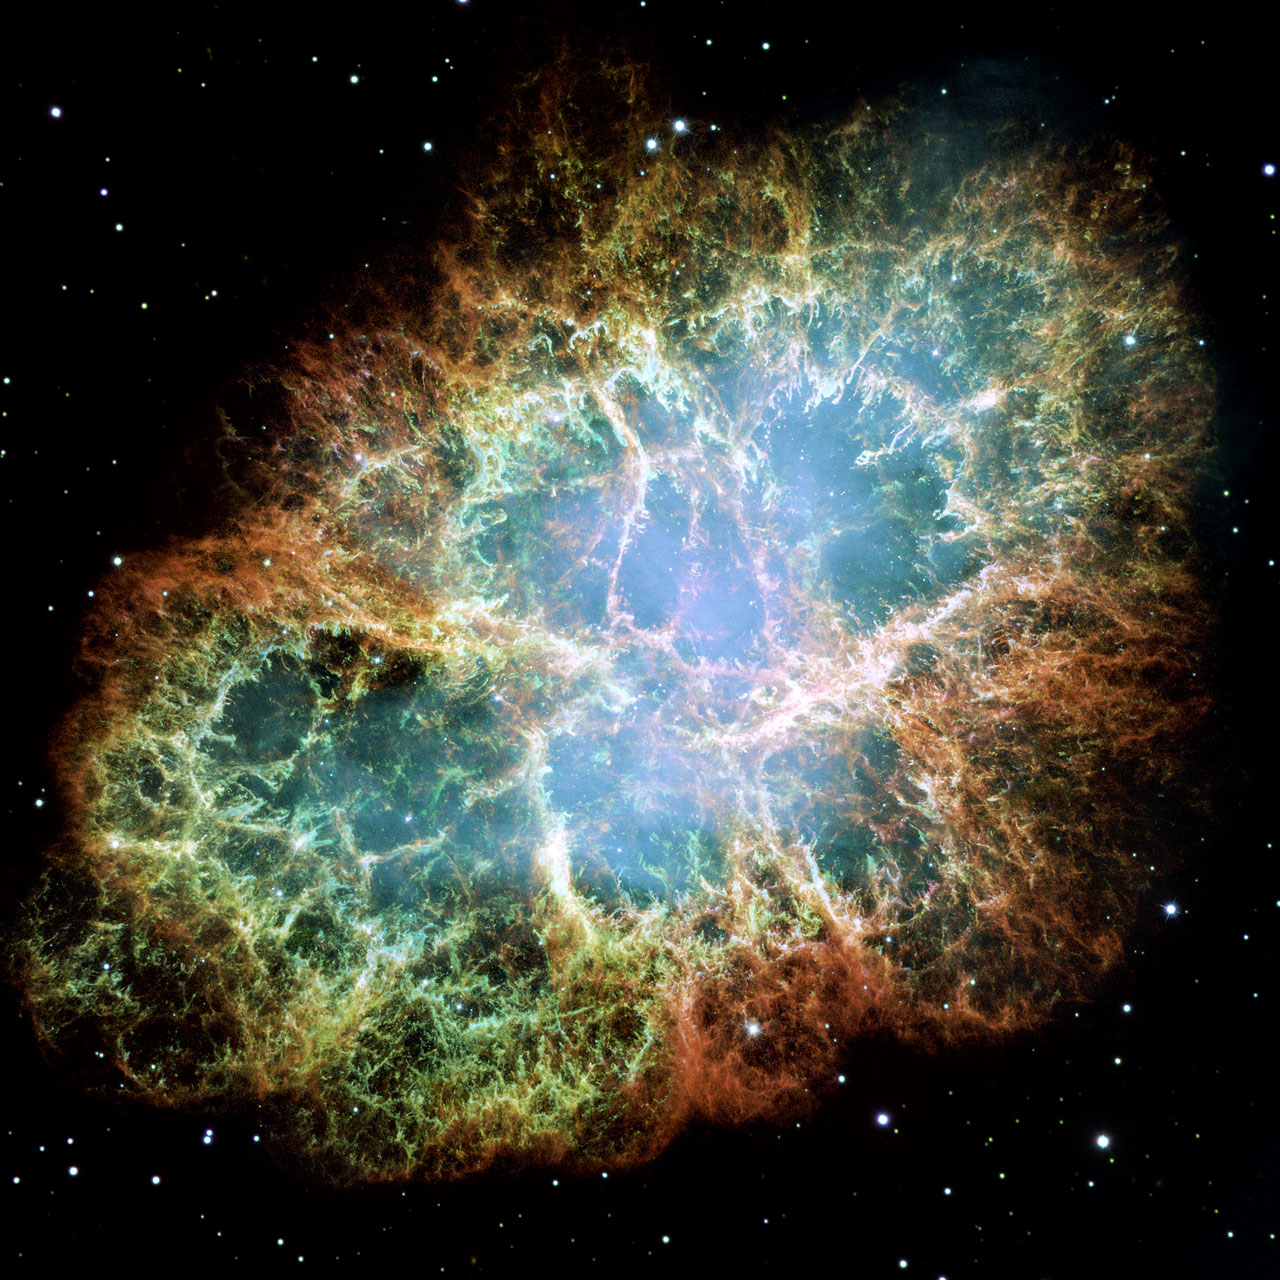
\includegraphics[width=\linewidth]{pictures/crab.jpg}
		\caption{Krebsnebel aufgenommen mit dem Hubble Teleskop.}%
    \label{fig:crab}
\end{wrapfigure}

In diesem Versuch wird der Krebsnebel untersucht.
Er ist ein Überrest einer Supernova-Explosion eines Sterns
mit 8~bis 12 Sonnenmassen beobachtet im Jahr 1054,
und befindet sich im Sternbild Stier.

Eine Supernova-Explosion ist das Ende eines massereichen Sterns,
bei der die Leuchtkraft eines Sterns kurzzeitig auf das millonen- bis
milliardenfache der ursprünglichen Leuchtkraft ansteigt,
ehe der Stern nach dem Verbrauch des
nuklearen Brennstoffs kollabiert und ein kompaktes Objekt
(Neutronenstern oder Schwarzes Loch) bildet.

Im Zentrum des Krebsnebels befindet sich ein Pulsar,
welcher die Quelle von starker elektromagnetischer Strahlung ist.
Pulsare sind schnell rotierende Neutronensterne,
welche sehr regelmäßige, kurze Pulse emittieren.
Typische Größen von Neutronensternen sind Durchmesser von einigen
\SI{10}{\kilo\meter}.
Die Materiereste, die bei einer Supernova-Explosion
vom zurückbleibenden Neutronenstern abgesprengt werden,
bilden eine überschallschnelle Schockwelle.
Diese heizt bei der Expansion das interstellare Medium auf Temperaturen von bis zu
\SI{e8}{\kelvin} auf.
Die propagierenden Schockwellen können durch Dichteschwankungen des stellaren
Mediums Sternbildung auslösen
und sind außerdem Lieferant für schwere Elemente, die in einem normalen
Fusionsprozess eines Sterns nicht gebildet werden können.
Der zurückbleibende Neutronenstern besitzt ein intensives Magnetfeld,
in dem hochenergetische Elektronen Synchrotonstrahlung erzeugen.
Des Weiteren kommt es zur Invers-Compton-Streuung,
bei dem ein hochenergetisches Elektron einen Teil seiner
Energie auf ein Photon überträgt.
Niederenergetische Photonen werden durch thermische Strahlung produziert.
Durch mehrfache Streuung und Synchrotonstrahlung entstehen so hochenergetische Gammateilchen,
die MAGIC detektieren kann.

Aufgrund seiner Eigenschaften wird er als Standardkerze der Gamma-Astronomie betitelt,
da der Teilchenfluss hier nahezu konstant und aufgrund der Nähe der Quelle vergleichsweise hoch ist.
% Durch seine Analyse kann die Performance von verschiedenen Teleskopen verglichen werden.
Mit Messdaten des Krebsnebels können unter Anderem Analysemethoden geprüft
oder die Performance verschiedener Detektoren verglichen werden.

\subsection*{Detektion}%
\label{sub:wobbelmodus}

% Da kosmische Quellen nicht isoliert von ihrer Umgebung betrachtet
% werden können,
% müssen zu jeder anvisierten Quellposition Umgebungsdaten aufgenommen werden.
% Die
% % wird zu jeder
% Quellposition heißt \textit{On}.
% % genau so lang Daten aufgenommen,
% % wie
% % und die
% Positionen nahe der Quellposition,
% in denen kein Gammafluss erwartet wird,
% heißen \textit{Off}.


Obwohl bei der Signal-Untergrund-Trennung ein großer Teil der hadronische Schauer aussortiert werden kann, bleibt
dennoch ein gewisser Anteil an Untergrund Ereignissen bestehen.
Da von einem
isotropen hadronischen Untergrund
innerhalb des Blickfeldes von MAGIC
ausgegangen werden kann,
ist eine Messung des Untergrundes an
einer äquivalenten Position ohne signifikante Gammaquelle möglich.
Somit kann
% in der Analyse der Untergrund von der Messung abgezogen werden, sodass nur das
in der Analyse ein Modell des Untergrundes an der Quellposition aus den
Messungen der Untergrundpositionen erstellt werden.
Ereignisse aus der Quellposition,
die dem Untergrundmodell ähnlich sehen, werden verworfen,
sodass nur noch das Signal (Exzess) übrig bleibt.
% Durch das Modell kann damit der Untergrund in der Quellposition zu minimiert werden,
% sodass nur das Signal (der Exzess) uebrigbleibt.
Die Quellposition heißt \textit{On}-Position, äquivalente Positionen ohne
Gammaquelle heißen \textit{Off}-Position.
Eine Möglichkeit wäre nun zwei Messungen durchzuführen: eine für die
Signalmessung an der On-Position und eine Untergrundmessung an einer
nahegelegenen Off-Position.


% Die Teleskope triggern drei Arten von Events.
% Neben den eigentlichen Luftschauern,
% welche durch Protonen
% oder Gammas verursacht werden,
% erzeugen Myonen oder versehentliche Trigger weitere Events.
% Myonen erzeugen ringförmige Ereignisse in der Kamera.
% Versehentliche Trigger entstehen z.B.\ durch den Nachthimmelhintergrund
% (\textit{Night Sky Background, NSB}) und elektronisches Rauschen.

% In der Gamma Ray Astronomie werden die Teleskope in der Regel auf einen Punkt
% ausgerichtet, an dem eine Quelle angenommen wird.
% Die gemessenen Events, die das Teleskop triggert, können vom
% kosmischen Hintergrund oder von einer echten Quelle, falls diese existiert, sein.

MAGIC nimmt Daten im Wobble-Modus auf.
Die erwartete Quellposition liegt dabei nicht im
Kameramittelpunkt,
sondern um
\SI{0.4}{\degree} um den Kameramittelpunkt
verschoben.
In äquidistanten Abständen um den Kameramittelpunkt
werden Off-Positionen bestimmt (siehe Abbildung~\ref{fig:hillas}).
Dies hat den Vorteil, dass die Aufnahme von On und Off Daten zeitgleich möglich
ist und so die Messzeit maximiert wird.

% Anschließend wird der Abstand $\theta$ der rekonstruierten
% zu der On- und den Off-Positionen bestimmt.
% Die Bins von $\theta^2$ werden in den Off-Positionen
% anhand der On-Position (Anzahl Off-Positionen / Messzeiten) normiert.
% Im Anschluss wird der aus den Off-Positionen bestimmte Untergrund
% aus der Messung der On-Position subtrahiert, sodass Signal übrig bleibt
% (vgl. Abbildung~\ref{fig:thetacut}).

\clearpage

  \section{MARS}%
\label{sec:mars}

\begin{wrapfigure}[31]{r}{0.5\textwidth}
  \centering
  \includegraphics[height=0.77\textheight]{tikz/build/overview.pdf}%
  \caption{Ü\-ber\-sicht der Ana\-lyse\-schrit\-te.}%
  \label{fig:uebersicht_analyse}
\end{wrapfigure}

MARS ist ein Software-Paket, das in \texttt{C++} geschrieben ist.
Es beinhaltet zum einen Container, um die aufgenommenen Daten zu speichern,
zum anderen viele Ausführbare,
mit denen die gesamte Analysekette für MAGIC durchgeführt wird.

Die Hauptprogramme werden im Folgenden näher erklärt.
Dabei sind sie so angeordnet, dass die Ergebnisse der einzelnen
Programme die Eingangsdaten der nächsten sind.

\subsection{Sorcerer}%
\label{sub:sorcerer}

Das Programm Sorcerer wird verwendet, um Rohdaten zu kalibrieren.
Es berechnet aus Lichtpulsen in den einzelnen PMTs eine Ankunftszeit und eine
Ladung.

\subsection{Star}%
\label{sub:star}
Ziel von Star ist die Berechnung von gereinigten Kamerabildern und die Berechnung
der Image Parameter auf den Daten.

\paragraph{Theorie}
Sobald das Teleskop ein Event triggert,
speichert es Daten von jedem PMT.\@
Diese Daten enthalten neben dem eigentlichen Tscherenkowlicht auch
Rauschen von elektronischen Bauteilen,
Nachthimmelhintergrund (NSB:\ Night Sky Background) z.B.\ des Mondes,
und andere Störungen.

\subparagraph{Image Cleaning}
Um sinnvoll die Image Parameter bestimmen zu können,
müssen die Daten bereinigt werden.
Dazu werden alle Pixel verworfen, die wahrscheinlich nicht zu den
vom Tscherenkowschauer ausgelösten Pixeln gehören.
Des Weiteren ist gutes Image Cleaning in der Lage,
% um einen konstanten Photostream zu bereinigen,
niederenergetische Ereignisse vom Untergrund zu trennen und damit
für einen geringen Energie-Schwellwert zu sorgen.

Zu jeder anvisierten Quellposition (\textit{On}) werden
genau so lang Daten aufgenommen,
wo kein Gammafluss (\textit{Off}) erwartet wird.
Da insbesondere der NSB abhängig von der Zeit und Quellposition ist,
müssen bei jeder Observation zusätzliche Off-Daten aufgenommen werden.

Das aktuell angewandte Image Cleaning heißt \textit{Sum Image Cleaning}.
Es besteht aus drei Schritten.
Zuerst werde die Pixel zu Clustern aus 2--4 nächsten Nachbarn zusammengefasst.
Es wird überprüft, ob die Summe an Photonen in einem Cluster
einen gewissen clustergrößenabhängigen Grenzwert übersteigt.
Ist dies der Fall, überstehen die Pixel das Cleaning.
Als zweites werden Schnitte auf der Ankunftszeit der so entstandenen
Pixel-Inseln gemacht.
Es werden die mittleren Ankunftszeiten jeder Insel bestimmt.
Weichen die Ankunftszeiten der Inseln zu stark von der Ankunftszeit der größten Insel ab,
werden die Pixel der Insel verworfen.
Pixel der übrigbleibenden Inseln werden im dritten Schritt gereinigt,
wobei zwei Grenzwerte $Q_{1} > Q_{2}$ existieren.
Im ersten Schritt wird geprüft,
ob die Pixel über dem
Grenzwert $Q_{1}$ liegen,
und ob sie einen Cluster mit mindestens zwei Pixeln bilden.
Ist dies der Fall,
werden zusätzlich angrenzende Pixel,
die über dem Grenzwert $Q_{2}$ liegen,
hinzugefügt.

Jeweils ein Beispiel für ein Kamerabild vor und nach dem Image Cleaning ist in
Abbildung~\ref{fig:cleaning} dargestellt.

\begin{figure}[htpb]
  \centering
  \begin{subfigure}[c]{0.48\linewidth}
    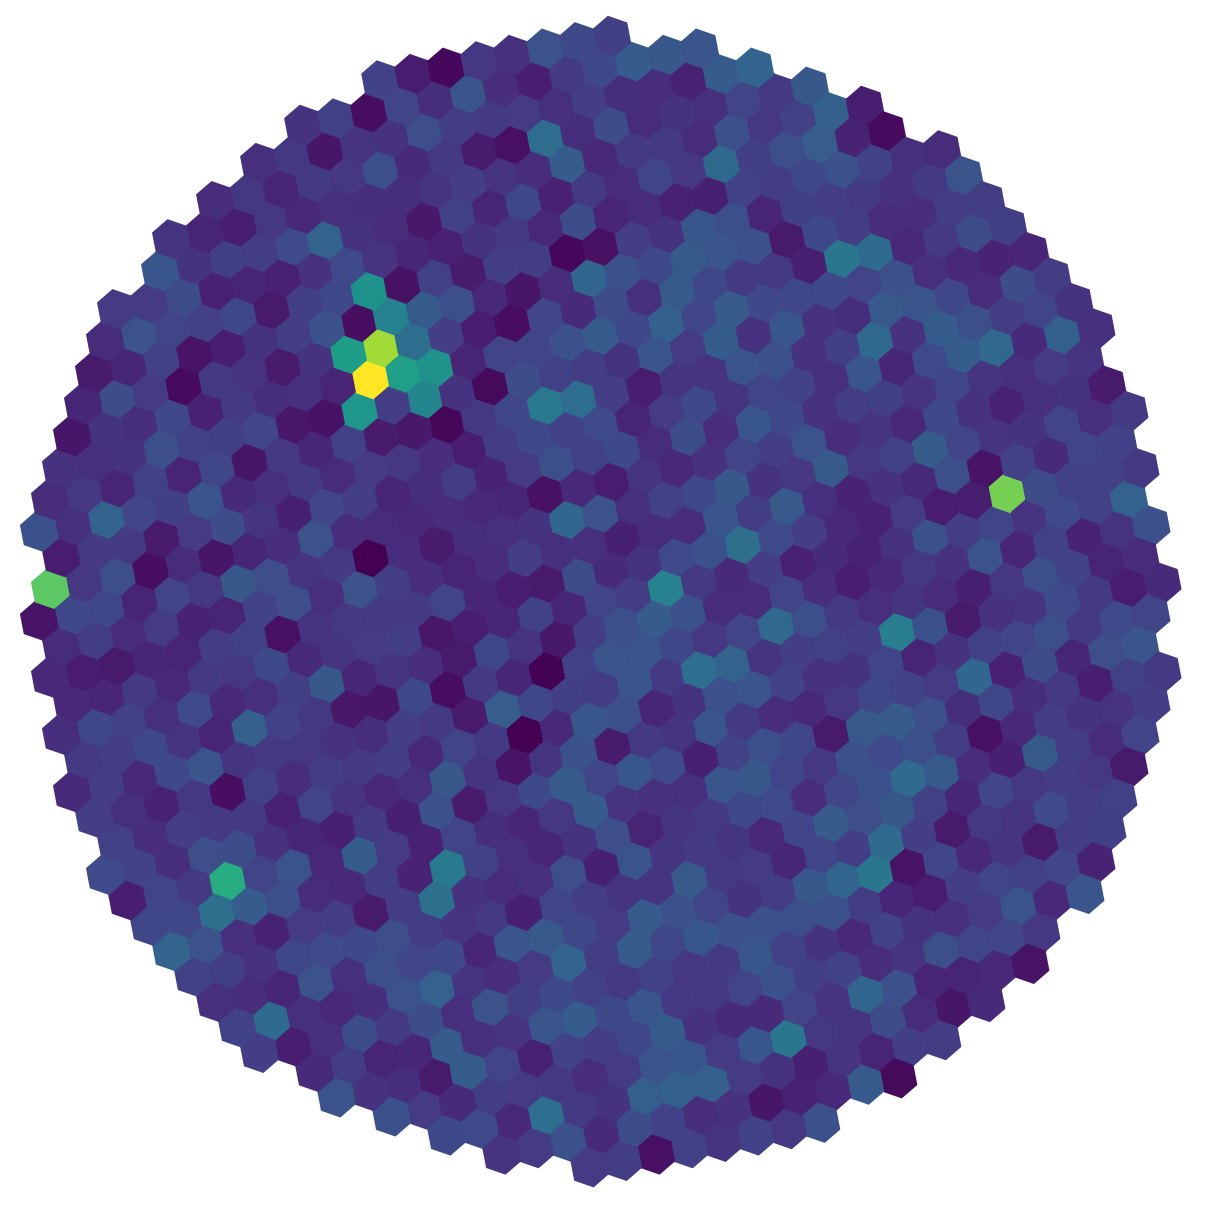
\includegraphics[width=\linewidth]{pictures/uncleaned.png}
    \caption{Kamerabild.}%
    \label{fig:uncleaned}
  \end{subfigure}
  \begin{subfigure}[c]{0.48\linewidth}
    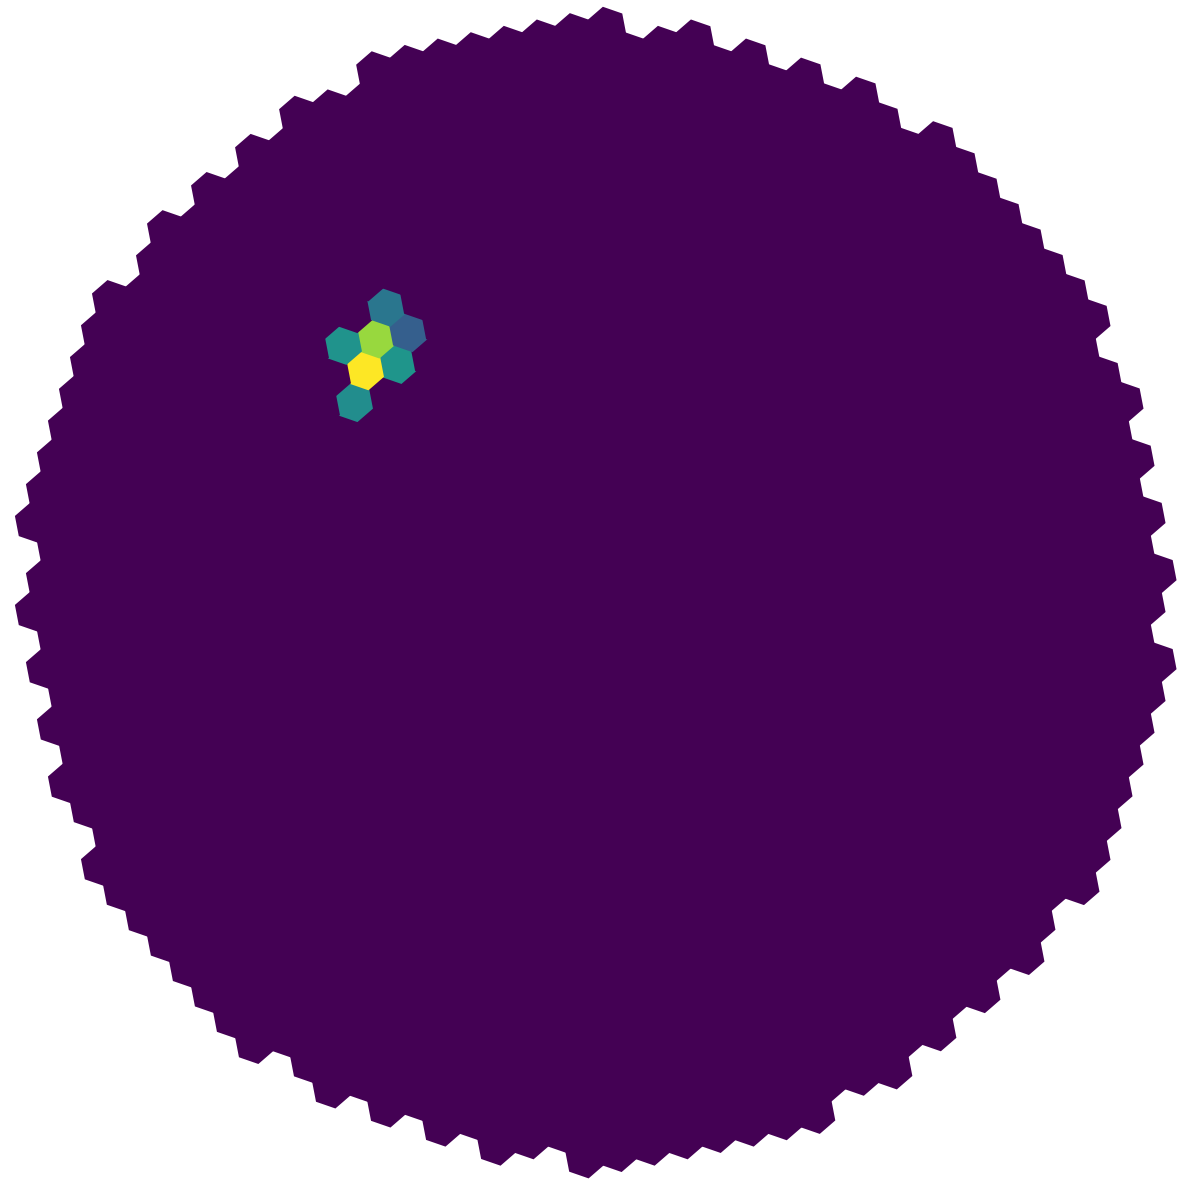
\includegraphics[width=\linewidth]{pictures/cleaned.png}
    \caption{Bereinigtes Kamerabild.}%
    \label{fig:cleaned}
  \end{subfigure}
  \caption{Bereinigung der Kamerabilder zur Berechnung der Image Parameter.}%
  \label{fig:cleaning}
\end{figure}

\subparagraph{Image Parameter}%
\label{spar:image_parameter}

Tscherenkowschauer erzeugen in der Kamera ellipsenförmige Events.
Unter anderem anhand der Größe der Ellipse und deren Ausrichtung
lässt sich die Energie des
Primärteilchens bestimmen und die Richtung rekonstruieren.
Dazu werden auf den gereinigten Kamerabildern die Image Parameter bestimmt.
Die Image Parameter entsprechen teilweise den Hillas Parametern,
und sind zweckmäßig erweitert.


\begin{wrapfigure}[15]{o}{0.4\textwidth}
  \centering
  \includegraphics[width=0.8\linewidth]{tikz/build/hillas.pdf}
  \caption{Image Parameter eines Schauers.}%
  \label{fig:hillas}
\end{wrapfigure}

Die Image Parameter \textit{length} und \textit{width} geben die Hauptachsen
der Ellipse an.
Da hadronische Schauer höhere transversale Entwicklung zeigen, ist
\textit{width} dazu geeignet, sie von Gammaschauern zu trennen.
\textit{Size} beschreibt die gesamte Anzahl an Photoelektronen im Schauerbild.
Die Anzahl an Photoelektronen verhält sich proportional zur Energie des
Primärteilchens.
\textit{CoG} (Center of Gravity) beschreibt den Schauerschwerpunkt im Kamerabild.
\textit{Conc-n} ist der Anteil der Photoelektronen in den $n$ hellsten Pixeln,
und beschreibt somit die Kompaktheit des Schauers.
Da gammainduzierte Schauer sehr kopmakt sind, ist dies auch eine gute
Trennvariable für Gamma/Handron-Separation.
\textit{Leakage1/2} beschreibt den Anteil des Signals in den \textit{1/2} äußeren
Pixelringen.
Dieser Parameter gibt eine Abschätzung,
ob Teile des Schauers außerhalb des Kamerabildes liegen.
\textit{Alpha} beschreibt den Winkel zwischen Hauptachse der Ellipse und
der Linie vom CoG zum Referenzpunkt (z.B.\ erwartete Quellposition).
Da gammainduzierte Schauer Richtung Quelle zeigen,
ist es ebenfalls ein trennstarker Parameter.
\textit{Dist} ist die Entfernung vom CoG zum Referenzpunkt.


\paragraph{Durchführung}

\subsection{Superstar}%
\label{sub:superstar}

Da MAGIC ein Stereoteleskop ist,
müssen die Daten beider Teleskope gemeinsam analysiert werden.
Superstar wird verwendet,
um die Image Parameter der gereinigten Daten beider
Teleskope zu einer Stereo-Parameter Datei zusammenzuführen.
Dabei werden weitere Parameter bestimmt,
die nur aus den Informationen beider Teleskope gewonnen werden können.

\paragraph{Theorie}%

\begin{wrapfigure}[12]{O}{0.4\textwidth}
  \centering
  \includegraphics[width=0.9\linewidth]{tikz/build/theta2.pdf}
  \caption{Stereoparameter eines Schauers.}%
  \label{fig:reco}
\end{wrapfigure}

Da die Quellposition in verschiedene Bereichen der beiden Kamerasensoren
liegt,
weise die Ellipsen unterschiedliche Orientierung auf.
Aus dem Schnittpunkt zweier Geraden,
die durch die Hauptachsen der Ellipsen gehen,
wird die rekonstruierte Quellposition bestimmt.

Auf die ähnliche Art wird über eine Koordinatentrafo vom Kamerasystem ins
Erdsystem der Aufprallpunkt des Schauers auf dem Erdboden
bestimmt.

% \textit{Height of shower max},
% \textit{Cherenkov radius},
% \textit{Cherenkov density},

Außerdem werden die Einzelergebnisse der beiden Teleskope verglichen,
um weitere Parameter zu bestimmen.
Für die \textit{Energy discrepancy} wird
ein $\chi^2$-Test durchgeführt,
wobei angenommen wird,
dass die wahre Energie in beiden Teleskopen identisch ist.
Die Richtungsrekonstruktionen beider Teleskope werden verglichen,
und die Differenz in \textit{DISP difference} gespeichert.

\subsection{Quate}%
\label{sub:quate}

Quate ist ein Programm,
das
% Mittelwerte von einem Parametersatz ausrechnet, und
Daten selektiert und in die Klassen \textit{gut} und \textit{schlecht} einteilt.
Durch das Aussortieren kann unter anderem gewährleistet werden,
dass sich die Daten der Monte Carlo-Simulation mehr mit den Messdaten decken.



% \paragraph{Theorie}%
% Hier ist einerseits das Problem, dass der Leser gar nicht weiss, was Monte Carlos sind und warum die mit den Daten uebereinstimmen muessen.

% Im Wetter koennen Daten und MCs nicht uebereinstimmen, weil das Wetter nicht mitsimuliert wird.

% Die gemessenen Daten werden nach Wetter selektiert, einfach um zu sehen, wie gut die Daten sind und ob ggf Korrekturen stattfinden muessen.

% Ausserdem braucht man in einer normalen Analyse Crab Daten, die den Messdaten besonders aehnlich in Zenit, Wetter, Mondbedingungen, etc sind. Hier natuerlich irrrelevant weil eh Crab :)

% Hadronische Daten werden nur fuer die gh Separation gebraucht und die sollen den Daten moeglichst aehnlich im Zenit sein.

% Soviel zum Verstaendnis. Aber da der Versuch ohne Quate durchgefuehrt wird: Kapitel weglassen! Eine allgemeine Erklaerung zu "welche Daten brauchen wir warum" wo das von oben drinsteht (ohne Wetter, nur was man wofuer braucht) Vielleicht direkt nach dem Schauerkapitel, wo eh noch der Satz zur gh Separation hinsoll...
% % \label{par:theorie}
Ziel der Analyse ist es, die Unsicherheiten z.B.\ des Flusses so gering wie
möglich zu halten.
Primärteilchen schauern in einer Höhe von \SIrange{10}{20}{\kilo\meter}
auf.
Da die Entwicklung des Schauers vom Dichteprofil der Atmosphäre abhängig ist,
ist es wichtig, dieses zu kennen.
Das Dichteprofil variiert abhängig vom Zenithwinkel und Wetter.
Daten und Monte Carlos müssen deshalb im Zenithbereich übereinstimmen.
% da die Weglänge durch die Atmosphäre entscheidend für die Schauerentwicklung ist.

% Weitere Instrumente, z.B. Lidar, messen Eigenschaften der Atmosphäre.
% Dazu misst Lidar die Lichttransmission.
% Ziel ist es, einen Datensatz zu erstellen,
% mit wenig variierenden und gut simulierbaren Wetterbedingungen.

% Die Wirkungsquerschnitte der Schauerprozesse sind dichteabhängig.
% Zur guten Rekonstruktion eines Schauers muss deswegen die Dichteverteilung
% bekannt sein.
% Dies Reduziert die Unsicherheiten auf die abgeleiteten Größen.

% % \paragraph{Durchführung}%

% % Das Programm \texttt{quate} wird über die
% % Datei \texttt{quate.rc} konfiguriert.
% % In dieser werden Einstellungen getroffen,
% % sodass die Daten sinnvoll prozessiert werden.
% % Dazu ist der Azimut und Zenit entsprechend der zu
% % observierenden Quelle einzustellen.
% % Dies ist über die Parameter \texttt{AzMin},
% % \texttt{AzMax}, \texttt{ZdMin} und \texttt{ZdMin}
% % möglich.
% % Zusätzlich ist der Parameter
% % \texttt{MinAerosolTrans9km = 0.8} anzupassen,
% % damit {\color{red}\ldots Aerosol \ldots} berücksichtigt wird.
% % Überlegen Sie sich,
% % bei welchen Daten das Selektieren sinnvoll ist
% % (On/Off/MC)
% % und führen Sie dieses durch.
% % Geben Sie dazu als \texttt{<INPUT-DIRECTORY>} die entsprechenden Pfade zu den Daten an.

% % \begin{lstlisting}
% %   quate -b -s -q \
% %     --stereo \
% %     --config=quate.rc \
% %     --out=<OUTPUT-DIRECTORY> \
% %     --ind=<INPUT-DIRECTORY>
% % \end{lstlisting}
% % Quate erstellt im \texttt{<INPUT-DIRECTORY>}
% % jeweils einen Ordner \texttt{bad} und \texttt{good},
% % in denen symbolische Links zu den jeweils ausgewählten Dateien liegen.
% % Dies ist für die folgenden Analyseschritte wichtig.

\subsection{Coach}%
\label{sub:coach}

Coach trainiert Modelle zur Separation von Signal und Untergrund,
sowie der Rekonstruktion von Energie und Richtung.

\paragraph{Theorie}%

\subparagraph{Gamma/Hadron-Separation}
Die Teleskope triggern drei Arten von Events.
Neben den eigentlichen Luftschauern,
welche durch Protonen
oder Gammas verursacht werden,
erzeugen Myonen oder versehentliche Trigger weitere Events.
Myonen erzeugen ringförmige Ereignisse in der Kamera.
Versehentliche Trigger entstehen z.B.\ durch NSB und elektronisches Rauschen.

Für die Analyse einer Quelle ist es wichtig,
das Signal (Gammaschauer) vom
Untergrund (alles andere) zu separieren.
Da Untergrundevents um mehrere Größenordnungen häufiger auftreten (1:\num{e5}),
geschieht dies durch ein multidimensionales maschinelles
Klassifizierungsystem (Random Forest).

\begin{wrapfigure}[18]{L}{0.6\textwidth}
  \centering
  \includegraphics[width=\linewidth]{build/hadroness.pdf}
  \caption{Schnitte auf der Hadroness und ihre Konsequenzen für die Analyse.}%
  \label{fig:uebersicht}
\end{wrapfigure}

Ziel des Modells ist es, Gammas den Wert 0 und Untergrund den Wert 1 zuzuweisen.
Dazu werden für unabhängige Entscheidungsbäume einer begrenzten Tiefe
der Informationsgehalt maximiert.
Durch Mittelung eines Events über alle trainierten Bäume entsteht ein Wert
zwischen eindeutig Gamma und eindeutig Hadron, welcher als Hadroness bezeichnet
wird.
Durch Schnitte auf diesem Wert kann eine Separation durchgeführt werden.

\subparagraph{Energierekonstruktion}%
\label{par:energie}

Die Energie des Gammas ist beinahe proportional
zur Anzahl der Tscherenkowphotonen
und somit der Photoelektronen in der Kamera,
jedoch hängt die Menge an detektiertem Licht von weiteren Parametern,
wie unter anderem Winkel der Kamera und Lage des Schauers im Kamerabild, ab.

In MARS wird die Energie des Primärteilchens auf zwei Arten rekonstruiert:
\begin{description}
	\item[\quad Look-up Tables] Für eine Look-up Table werden Monte Carlo
		Gammas in ausgewählten Parametern gebinnt.
		Diesen Bins wird eine mittlere Energie aller
		zugehörigen Gammas zugewiesen.
		Bei realen Events werden die Parameter mit der Tabelle verglichen
		und so eine Energie geschätzt.
		Es muss darauf geachtet werden,
		dass die Bins möglichst homogen und mit ausreichend Statistik gefüllt sind.
	\item[\quad Random Forest] Außerdem wird eine Random Forest Regression (s.o.)
		zur Bestimmung der Energie durchgeführt.
\end{description}

\subparagraph{Richtungsrekonstruktion}%
\label{par:position}

Die Rekonstruktion der ursprünglichen Richtung ist einer der Hauptziele.
Dafür werden nach der ersten Abschätzung in Kapitel~\ref{sub:superstar} weitere
Analyseschritte durchgeführt.
Dazu wird zunächst die \textit{DISP (\textbf{D}istance between the
\textbf{I}mage controid and the \textbf{S}ource \textbf{P}osition)} bestimmt.
Diese gibt die Entfernung vom Schauerschwerpunkt zur rekonstruierten Quellposition
entlang der Hauptachse der Ellipse an (siehe Abbildung~\ref{fig:reco}).
Das Vorzeichen des DISP-Parameters ist nicht bestimmt,
sodass es zwei mögliche Quellpositionen gibt.
Da MAGIC ein Stereoteleskop ist,
kann bei der Schätzung des Vorzeichens des DISP-Parameters
der Schnittpunkt der beiden Hauptachsen als zusätzliche Information
verwendet werden.
Die rekonstruierte Position wird möglichst nah an dem Schnittpunkt der Achsen
gewählt, was den Vorteil birgt,
dass ca.\ 10--20\% schlecht rekonstruierte Events verworfen werden.
Die Schätzung des DISP-Parameters wird momentan über einen Random-Forest
getätigt, wo Informationen wie die Momente entlang der
Hauptachse oder der Zeitgradient eingehen.
Hadronische Schauer, welche fälschlicherweise die Gamma/Hadron-Separation
überstanden habe, weisen meist eine schlechte Richtungsrekonstruktion auf.

\paragraph{Durchführung}%
In der \texttt{coach.rc} sind die Pfade
\texttt{RF.mcdata},
\texttt{RF.data},
und \texttt{RF.outpath}
anzupassen.
Es sollen hier die Rootfiles mittels Wildcards angegeben werden
(Bsp.: \texttt{*.root}).
Die Monte Carlo Daten sind in einen Trainingsdatensatz
und einem Testdatensatz aufgeteilt.
Die Trainingsdaten sind durch die Endung
\texttt{*\_wr\_1.root} gekennzeichnet.
Desweiteren ist der Zenit sinnvoll einzustellen.
Zur schnelleren Erzeugung von Ergebnissen kann die Anzahl an
Entscheidungsbäumen auf \num{50}
reduziert werden.
Es sind die Argumente
\texttt{-RFgh}, \texttt{-LUTs}, und \texttt{-RFdisp}
zum Erstellen eines Random Forest für die Gamma-/Hadron-Separation,
einer Look-Up-Table für die Energieschätzung,
und eines weiteren Random Forest für zusätzliche Energieschätzung.

\begin{lstlisting}
  coach -q -b	\
    --config=coach.rc \
    -RFgh \
    -LUTs \
    -RFdisp
  # oder parallel zur schnelleren Rechnung:
  coach -q -b --config=coach.rc -RFgh
  coach -q -b --config=coach.rc -LUTs
  coach -q -b --config=coach.rc -RFdisp
\end{lstlisting}

Es werden fünf Dateien erzeugt,
die als weitere Eingangsdaten für die folgenden Analyseschritte verwendet
werden.

\subsection{Melibea}%
\label{sub:melibea}



\subsection{Odie}%
\label{sub:odie}

\paragraph{Theorie}%
\begin{equation}
	S = \sqrt{2} \left(
		N_\text{on} \log \left[
			(\tau + 1) \left( 
				\frac{N_\text{on}}{N_\text{on} + N_\text{off}} 
			\right)
		\right]  
		+ N_\text{off} \log \left[
			\left( \frac{1 + \tau}{\tau} \right) \left( 
				\frac{N_\text{off}}{N_\text{on} + N_\text{off}} 
			\right)
		\right]  
	\right) ^ {1/2}
\end{equation}


\paragraph{Durchführung}%

Die Konfigurationsdatei \texttt{odie.rc} wird verwendet.
Es muss das Feld \texttt{Odie.dataName} angepasst werden.
Es gilt wieder, mit Wildcards die von Melibea prozessierten Daten zu nutzen
(Bsp.: \texttt{*\_Q\_*.root}).

\begin{lstlisting}
	odie -q -b --config=odie.rc
\end{lstlisting}

\subsection{Caspar}%
\label{sub:caspar}

% Skymaps sind Grundlage einer jeden Datenanalyse
% und sind von besonderem Interesse bei ausgedehnten Quellen,
% oder bei vorhandenseien anderer Quellen im FoV.

Skymaps dienen zur Visualisierung der Messdaten und sind von besonderem
Interesse, um zu überprüfen, ob sich (weitere) Quellen im Blickfeld befinden
oder die Quelle an sich ausgedehnt ist.

\paragraph{Theorie}%

Eine Skymap ist eine zweidimensionale Repräsentation der aufgenommen Ereignisse.
Ziel ist es, den gemessenen Events eine Position zuzuordnen.
Dazu werden ge\-wöhn\-lich drei verschieden Koordinatensysteme genutzt:

\begin{description}
  \item[\quad Kamera Koordinaten] werden genutzt, um die Sensitivität des
    Teleskops
    als eine Funktion in der Kamera zu beschreiben.
    Eine Repräsentation ist in Abbildung~\ref{fig:cleaning} zu sehen.
    Anhand dieser lassen sich beispielsweise Inhomogenitäten,
    wie sie ein helle Quelle verursacht, bereinigen.
  \item[\quad Azimuthal Koordinaten] sind abhängig von der Position des
    Beobachters auf der Erde.
    Sie sind nicht für die Observation von Astronomischen Objekten von Nutzen,
    aber um die Performance zu testen.
    Dazu werden Daten bei verschiedenen Zenitwinkel verglichen,
    was eine Variation der Atmosphärendicke entspricht.
  \item[\quad Äquatorial Koordinaten] werden genutzt, um eine Skymap einer astrophysikalischen Quelle anzufertigen.
\end{description}

\begin{wrapfigure}[10]{O}{0.36\textwidth}
  \centering
  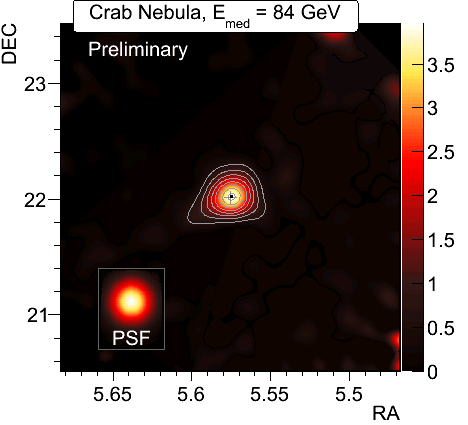
\includegraphics[width=\linewidth]{pictures/skymap.png}
  \caption{Skymap einer Beobachtung des Krebsnebels.}%
  \label{fig:skymap}
\end{wrapfigure}

Die Anfertigung einer Skymap ist nicht so simpel wie bei einem gewöhnlichen
Bild.
Für eine Skymap reicht nicht allein die Konstruktion eines 2D-Arrays,
bei dem die Information allein im Signalverlauf der Pixel enthalten ist,
wie es bei gewöhnlichen Bildern der Fall ist.

Vielmehr wird für jedes Gammaevent ein einzelnes Bild aufgenommen,
auf dem die Richtung rekonstruiert wird.
Eine Skymap bildet eine Menge an rekonstruierten Richtungen im Himmel ab.
Da die Auflösung des Detektors beschränkt ist,
schmieren die rekonstruierten um die wahren Quellposition aus.
Das Ausschmieren der Quelle wird durch die \textit{Point Spread Function (PSF)}
beschrieben
und kann auf einer Skymap bestimmt werden.
Durch die PSF kann das Auflösungsvermögen eines Teleskops
beschrieben werden und bildet daher eine wichtige Größe.

\paragraph{Durchführung}%

Die Konfigurationsdatei \texttt{caspar.rc} wird verwendet.
Es muss das Feld \texttt{Caspar.dataName} angepasst werden.
Wie bei Odie werden die von Melibea prozessierten Daten genutzt.

\begin{lstlisting}
  caspar -q -b --config=caspar.rc
\end{lstlisting}

Caspar erzeugt die Datei \texttt{Output\_caspar.root}.

\subsection{Flute}%
\label{sub:flute}
Ziel von Flute ist,
es das Energiespektrum und die Lichtkurve einer Quelle zu bestimmen.

\paragraph{Theorie}%
\label{par:theorie}

Zur Berechnung werden die Anzahl an detektiereten Gamma-Rays,
die effektive Observationszeit,
und die Collecting Area des Teleskop benötigt.

\begin{equation}
\frac{\text{d} \Phi}{\text{d}E} \simeq K {\left( \frac{E}{E_0} \right)}^{- \Gamma}
\end{equation}


\paragraph{Durchführung}%

Die Konfigurationsdatei \texttt{flute.rc} wird verwendet.
Es müssen die Felder \texttt{flute.data} und \texttt{flute.mcdata} angepasst werden.
Es werden die von Melibea prozessierten Daten und Monte Carlos genutzt.


\begin{lstlisting}
  flute -q -b --config=flute.rc
\end{lstlisting}

\subsection{CombUnfold}%
\label{sub:combunfold}
\paragraph{Theorie}%
\label{par:theorie}

\begin{equation}
	g(y) = \int_\text{c}^\text{d} M(x,y) f(x) \text{dx} + b(y)
\end{equation}

\begin{equation}
	g_i = \sum_j M_{ij} f_j + b_i
\end{equation}

\begin{equation}
	g_i = \int_{y_{i-1}}^{y_i} g(y) \text{dy} \quad \text{und} \quad
	b_i = \int_{y_{i-1}}^{y_i} b(y) \text{dy}
\end{equation}



\end{document}
